% https://tex.stackexchange.com/a/461325
\documentclass{beamer}

\usepackage{tikz}

\begin{document}

\begin{frame}
\begin{columns}[onlytextwidth]
\begin{column}{.25\textwidth}
a

b
\end{column}
\begin{column}{.1\textwidth}
$\Leftarrow$
\end{column}
\begin{column}{.25\textwidth}
a

b
\end{column}
\begin{column}{.1\textwidth}
$\Leftarrow$
\end{column}
\begin{column}{.25\textwidth}
a

b
\end{column}
\end{columns}

\bigskip

\begin{columns}[onlytextwidth]
\begin{column}{.25\textwidth}
I

L
\end{column}
\begin{column}{.1\textwidth}
\end{column}
\begin{column}{.25\textwidth}
\end{column}
\begin{column}{.1\textwidth}
\end{column}
\begin{column}{.25\textwidth}
\end{column}
\end{columns}


\begin{tikzpicture}[remember picture, overlay]
\draw[red] (0.5,1) circle (1);
\end{tikzpicture}

\end{frame}



\end{document}
